\documentclass{article}

\usepackage{graphicx}
\usepackage{listings}
\usepackage{hyperref}

\setlength{\textwidth}{6.7in}
\setlength{\oddsidemargin}{-0.1in}
\setlength{\textheight}{8.6in}
\setlength{\topmargin}{-0.4in}

\title{Meeting with Dom 20210217}
\author{Lena Morrill}
\date{\today}

\begin{document}
\maketitle

\section{Links}

\begin{itemize}
\item \href{https://www.overleaf.com/project/5e6fb59b1abb040001d1352b}{Link to paper}
\item \href{https://github.com/lm687/Global_Differential_Abundance_Pipeline}{Link to github repo}
\item \href{https://github.com/lm687/Global_Differential_Abundance_Pipeline/blob/master/code/3_analysis/simulation_model_assessment/generate_datasets_simulations/GenerationCnorm.R}{Script simulating data under the model}
\end{itemize}

\section{State of the inference}
Convergence of PCAWG samples in full-RE multinomial model

\begin{itemize}
\item The vast majority of samples have not converged (see Figure \ref{convergence}). This also happens with simulated datasets, sometimes. (\texttt{Hessian of fixed effects was not positive definite.})
\item This is especially the case for signatures (as opposed to the six nucleotide substitutions)
\item signatures are, in general, more than 6, so if the problem is that there are too many categories and too few samples to converge properly, this would explain it
\item The problem in inference is that the gradient is too steep. However, despite being the fixed effects covariance matrix being non-pd, the simulated data from these models (with the inferred parameters) show a very good correlation with the observed data (could it be that there is a problem with identifiability meaning that parameters are highly correlated?)
\item Sometimes changing the initial conditions is enough to have a good convergence
\item Another possibility is that signatures with very low abundance are the problem, and that we should remove those prior to analysing the exposures
\item Another possibility is that the last category (signature), which is the one used as baseline, is very low in certain cancer types, and this doesn't allow good inference
\item Using Head-SCC with signatures as an example, I am showing that using a subset of the exposures leads to correct, non-pd, inference, when using a full-RE multinomial
\item Using simulated data, I see that even if convergence isn't good, the parameters are quite well recovered
\end{itemize}

\section{My questions for Dom}
\begin{enumerate}

\item What does this do exactly. My params are not well recovered unless the  \verb|opt <- do.call("optim", obj)|
part is called, but \verb|rep <- sdreport(obj)| does not take any arguments that have to do with this!

\begin{lstlisting}
obj <- MakeADFun(data = TMB_data_sim, parameters = TMB_params_sim,
            DLL="tmb_MVN_partial_ILR", random = "u_large")
opt <- do.call("optim", obj)
opt
opt$hessian ## <-- FD hessian from optim
rep <- sdreport(obj)
rep
\end{lstlisting}

\item If we're integrating over the random effects, doesn't that mean that the \verb|log_sd|, cov from the RE should not be inferred? what exactly are the RE values that TMB spits out? are they the values from the best fit? check that way I integrate out the multivariate random effects is done correctly

\item DM vs categorical. I was wondering how individual mutations add to the likelihood. In DM or M, samples with more mutations will have a lower weight in the neighbourhood because the multinomial coefficient increases rapidly with the number of draws. However, what I had thought initially is that samples with a larger number of mutations should contribute \emph{more} to the likelihood than samples with fewer mutations (and this scenario corresponds to the categorical distribution, as I understand it). Is there an overdispersed version of the categorical (analogous to the Dirichlet-Multinomial)? Link to the script for the \href{https://github.com/lm687/Global_Differential_Abundance_Pipeline/blob/master/code/2_inference_TMB/mm_multinomial/fullRE_ME_multinomial.cpp}{multinomial fit} and the \href{https://github.com/lm687/Global_Differential_Abundance_Pipeline/blob/master/code/2_inference_TMB/mm_multinomial/fullRE_ME_multinomial_categorical.cpp}{categorical fit}.

\begin{figure}[h]
\centering
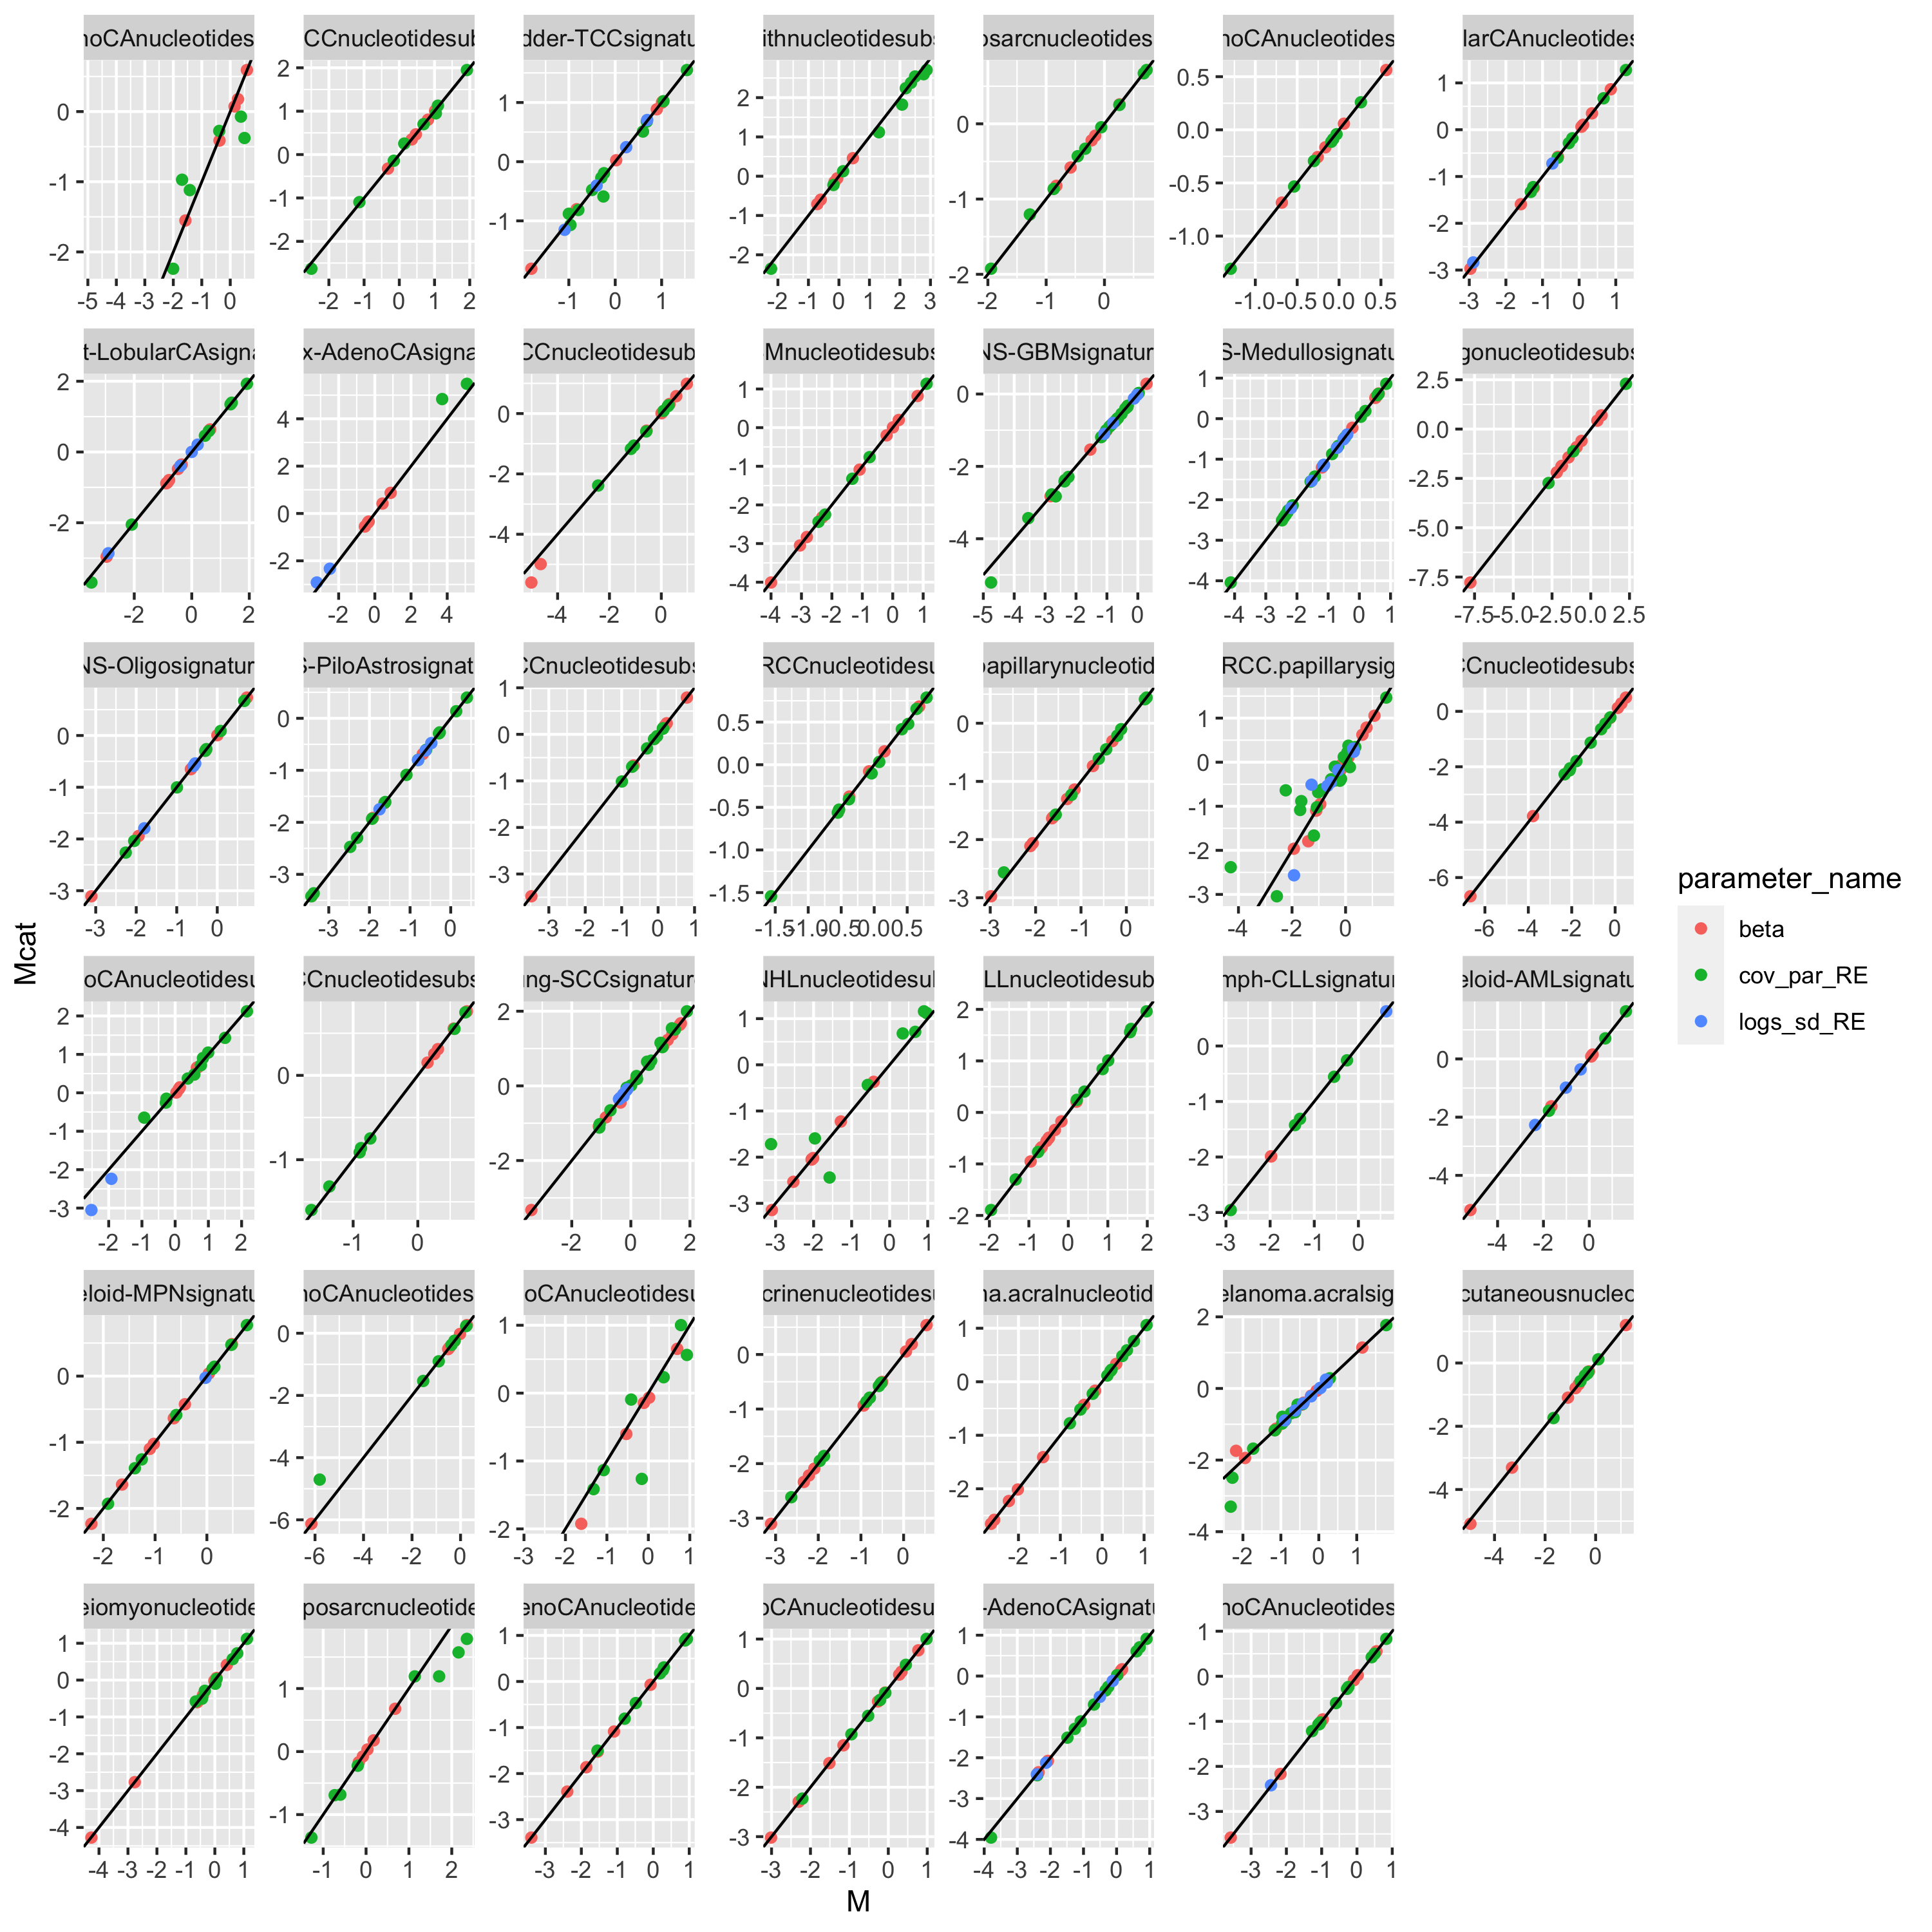
\includegraphics[width=3in]{figures/M_vs_catM_scatter.png}
\caption{The estimates for the multinomial fit and the categorical fit are extremely similar, even though the number of mutations per sample varies quite a lot, which I would expect to be reflected in the estimates}
\end{figure}

\end{enumerate}

\begin{figure}[h]
\centering
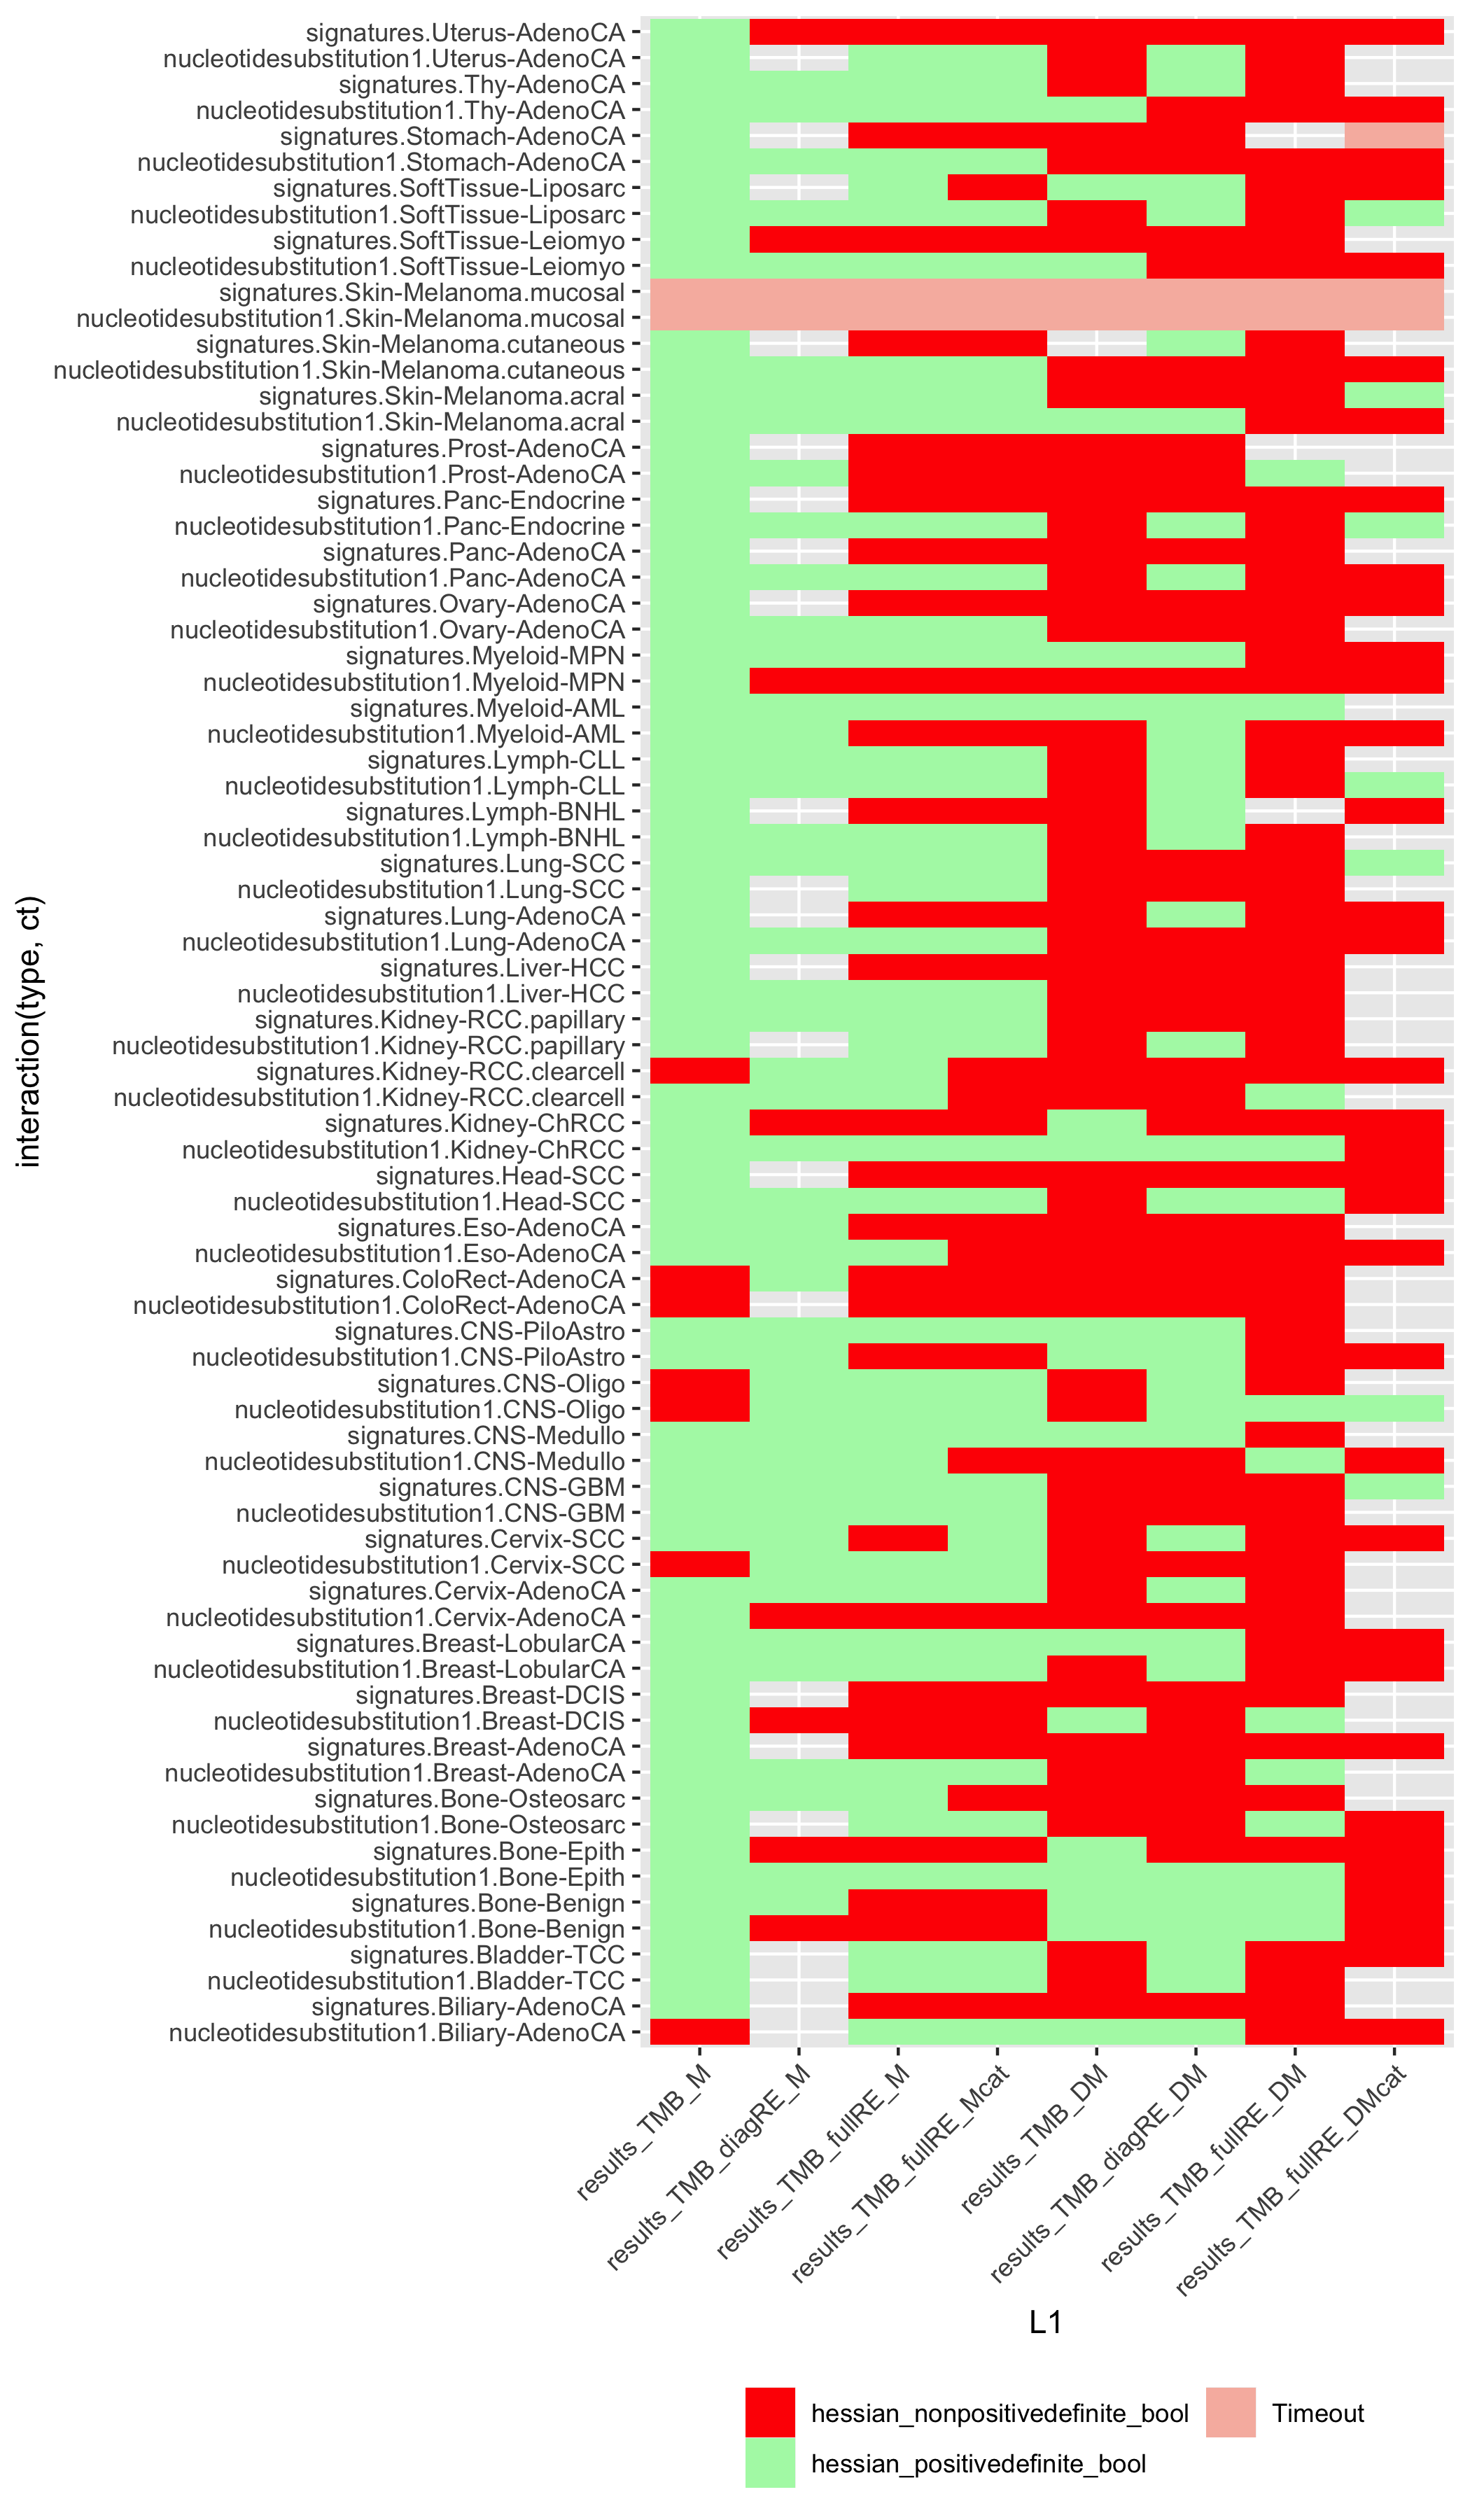
\includegraphics[width=.7\textwidth]{/Users/morril01/Documents/PhD/GlobalDA/results/results_TMB/pcawg/summary_runs.png}
\caption{Convergence of PCAWG samples \label{convergence}}
\end{figure}

\begin{figure}[h]
\centering\includegraphics[width=.49\textwidth]{/Users/morril01/Desktop/pairs_CNS-Medullo_signatures_MfullRE_stan.png}
\includegraphics[width=.49\textwidth]{/Users/morril01/Desktop/pairs_ColoRect-AdenoCA_signatures_MfullRE_stan.png}
\caption{Pairs plot of the posteriors for the fullRE M for a sample that has converged with TMB (left; CNS-Medullo signatures) and one that hasn't (right; ColoRect-AdenoCA signatures). Yellow dots indicate transitions that hit the maximum treedepth.}
\end{figure}

\end{document}